% Status info:
% M. Gates	2006-2009
% A. Wolf	2011-2014
% B. Gerdes	2013
% Additions inserted from wiki 2015-12-26
% Content OK for 0.12.4.
% 2016-04 GZ started restructuring
% TODO: typo&grammar check

%\chapterimage{chapter-t2-bg} % Chapter heading image (now in guide.tex)

\chapter{A First Tour}
\label{ch:tour}


\begin{figure}[tbh]\centering
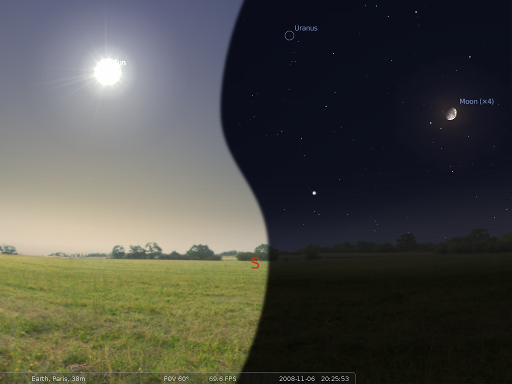
\includegraphics[width=0.95\textwidth,trim=0 0 0 30,clip]{001.png}
\caption{Stellarium main view. (Combination of day and night views.)}
\label{fig:001}
\end{figure}

\noindent When Stellarium first starts, we see a green meadow under a
sky. Depending on the time of day, it is either a day or night
scene. If you are connected to the Internet, an automatic lookup will
attempt to detect your approximate position.\footnote{See
  section~\ref{sec:gui:location} if you want to switch this off.}

At the bottom left of the screen, you can see the status bar. This shows
the current observer location, vertical field of view (FOV), graphics performance
in frames per second (FPS) and the current simulation date and time.
If you move the mouse over the status bar, it will move up to reveal a
tool bar which gives quick control over the program.

The rest of the view is devoted to rendering a realistic scene including
a panoramic landscape and the sky. If the simulation time and observer
location are such that it is night time, you will see stars, planets and
the moon in the sky, all in the correct positions.

You can drag with the mouse on the sky to look around or use the
cursor keys. You can zoom with the mouse wheel or the \key{Page
  \arrowkeyup} or \key{Page \arrowkeydown} keys.

Much of Stellarium can be controlled very intuitively with the
mouse. Many settings can additionally be switched with shortcut keys
(hotkeys).  Advanced users will learn to use these shortcut
keys. Sometimes a key combination will be used. For example, you can
quit Stellarium by pressing \key{\ctrl+Q} on Windows and Linux, and
\key{\cmdmac+Q} on Mac OS X.  For simplicity, we will show only the
Windows/Linux version. We will present the default hotkeys in this
guide. However, almost all hotkeys can be reconfigured to match your
taste. Note that some listed shortkeys are only available as key
combinations on international keyboard layouts, e.g., keys which
require pressing \key{AltGr} on a German keyboard. These must be
reconfigured, please see~\ref{sec:gui:help:hotkeys} for details.


The way Stellarium is shown on the screen is primarily governed by the
menus. These are accessed by dragging the mouse to the left or bottom
edge of the screen, where the menus will slide out. In case you want
to see the menu bars permanently, you can press the small buttons
right in the lower left corner to keep them visible.


\section{Time Travel}
\label{sec:tour:timeTravel}

When Stellarium starts up, it sets its clock to the same time and date
as the system clock. However, Stellarium's clock is not fixed to the same
time and date as the system clock, or indeed to the same speed. We may
tell Stellarium to change how fast time should pass, and even make time
go backwards! So the first thing we shall do is to travel into the
future! Let's take a look at the time control buttons on the right hand
ride of the tool-bar. If you hover the mouse cursor over the buttons, a
short description of the button's purpose and keyboard shortcut will
appear.

\begin{table}[h]
\centering
\begin{tabular}{ccl}\toprule
\emph{Button} & \emph{Shortcut key} & \emph{Description}\\\midrule
\guibutton[0.75]{2.25}{bt_timerate_decrease.png} & \key{J} & Decrease the rate at which time passes \\
\guibutton[0.75]{2.25}{bt_timerate_normal.png}   & \key{K} & Make time pass as normal \\
\guibutton[0.75]{2.25}{bt_timerate_increase.png} & \key{L} & Increase the rate at which time passes \\
\guibutton[0.75]{2.25}{bt_time_normal.png}       & \key{8} & Return to the current time \& date \\
\bottomrule
\end{tabular}
\caption{Time Travel}
\end{table}

OK, so lets go see the future! Click the mouse once on the increase time
speed button \guibutton{0.6}{bt_timerate_increase.png}. 
Not a whole lot seems to happen. However, take a look at the clock in
the status bar. You should see the time going by faster than a normal
clock! Click the button a second time. Now the time is going by faster
than before. If it's night time, you might also notice that the stars
have started to move slightly across the sky. If it's daytime you might
be able to see the sun moving (but it's less apparent than the movement
of the stars). Increase the rate at which time passes again by clicking
on the button a third time. Now time is really flying!

Let time move on at this fast speed for a little while. Notice how the
stars move across the sky. If you wait a little while, you'll see the
Sun rising and setting. It's a bit like a time-lapse movie. 

Stellarium not only allows for moving forward through time -- you can
go backwards too! Click on the real time speed button
\guibutton{0.6}{bt_timerate_normal.png}.  The stars and/or the
Sun should stop scooting across the sky. Now press the decrease time
speed button \guibutton{0.6}{bt_timerate_decrease.png} once. Look
at the clock. Time has stopped. Click the decrease time speed button
four or five more times. Now we're falling back through time at quite
a rate (about one day every ten seconds!).

\subsection*{Time Dragging, Time Scrolling}
\label{sec:tour:timeDrag}

Another way to quickly change time is \indexterm{time dragging}. Press
\keys{\ctrl}, press the left mouse button, and slide the mouse along the direction of daily motion to go forward, 
or to the other direction to go backward.

\newFeature{0.15.1}Similarly, pressing \keys{\ctrl} and scrolling the mouse wheel will 
advance time by minutes, pressing \keys{\ctrl+\shift} and 
scrolling the mouse wheel will advance time by hours, \keys{\ctrl+\Alt} by days, 
and finally \keys{\ctrl+\shift+\Alt} by calendar years.


Enough time travel for now. Wait until it's night time, and then click
the real time speed button \guibutton{0.6}{bt_timerate_normal.png}.
If all works as intended you will now be looking at the night sky.

\section{Moving Around the Sky}
\label{sec:tour:moving}

\begin{table}[h]
\centering
\begin{tabular}{ll}\toprule
\emph{Key}                         & \emph{Description}\\\midrule
Cursor keys \keys{\arrowkeyleft} \keys{\arrowkeyright} \keys{\arrowkeyup} \keys{\arrowkeydown} & Pan the view left, right, up and down \\
\keyPageUp{}/\keyPageDown{}, \keys{\ctrl+\arrowkeyup}/\keys{\ctrl+\arrowkeydown} & Zoom in and out \\
Left mouse button                  & Select an object in the sky \\
Right mouse button, \key{\ctrl+\space} & Clear selected object \\
Centre mouse button (wheel press)  & Centre selected object and start tracking \\
Mouse wheel                        & Zoom in and out \\ 
\key{\space}                       & Centre view on selected object \\
Forward-slash (\key{/})            & Auto-zoom in to selected object \\
Backslash (\key{\textbackslash{}}) & Auto-zoom out to original field of view \\\midrule
\key{\shift+N}                     & Look towards North (keep altitude)\\
\key{\shift+E}                     & Look towards East (keep altitude)\\
\key{\shift+S}                     & Look towards South (keep altitude)\\
\key{\shift+W}                     & Look towards West (keep altitude)\\
\key{\shift+Z}                     & Look towards Zenith (south down)\\
\key{\Alt+\shift+N}                & Look towards North Celestial Pole\\
\key{\Alt+\shift+S}                & Look towards South Celestial Pole\\
\bottomrule
\end{tabular}
\caption{Moving Around the Sky}
\label{tab:tour:moving}
\end{table}

As well as travelling through time, Stellarium lets you look around the
sky freely, and zoom in and out. There are several ways to accomplish
this, listed in table~\ref{tab:tour:moving}.

Let's try it. Use the cursors to move around left, right, up and down.
Zoom in a little using the \keyPageUp{} key, and back out again using the
\keyPageDown{}. Press the \key{\textbackslash} key and see how Stellarium returns to the
original field of view (how ``zoomed in'' the view is), and direction of
view.
%% TODO Is this still original behaviour? On German Kbd, this does not work anyways, backslash is a AltGr-combination.

If you prefer stepwise zooming to fixed values for field of view,
table~\ref{tab:FOVkeys} lists the keys to reach a certain field of
view.

\begin{table}[tb]
\centering
\begin{tabular}{lr||lr}\toprule
\emph{Hotkey} & \emph{Field of view}&\emph{Hotkey} & \emph{Field of view}\\\midrule
 \key{\ctrl+\Alt+1}&180$\degree$ & \key{\ctrl+\Alt+6}& 10$\degree$\\
 \key{\ctrl+\Alt+2}& 90$\degree$ & \key{\ctrl+\Alt+7}& 5$\degree$ \\
 \key{\ctrl+\Alt+3}& 60$\degree$ & \key{\ctrl+\Alt+8}& 2$\degree$ \\
 \key{\ctrl+\Alt+4}& 45$\degree$ & \key{\ctrl+\Alt+9}& 1$\degree$ \\
 \key{\ctrl+\Alt+5}& 20$\degree$ & \key{\ctrl+\Alt+0}& 0.5$\degree$ \\\bottomrule
\end{tabular}
\caption{Hotkeys to set fixed vertical fields of view}
\label{tab:FOVkeys}
\end{table}


Most users prefer to move around using the mouse. If you left-click
and drag somewhere on the sky, you can pull the view around.

Another method of moving is to select some object in the sky (left-click
on the object), and press the \key{Space} key to centre the view on that
object. Similarly, selecting an object and pressing the forward-slash
key \key{/} will centre on the object and zoom right in on it.

The forward-slash \key{/} and backslash \key{\textbackslash} keys auto-zoom in and out to different
zoom levels depending on what is selected. If the object selected is a planet
or moon in a \emph{sub-system} with a lot of moons (e.g.\ Jupiter), the
initial zoom in will go to an intermediate level where the whole
sub-system should be visible. A second zoom will go to the full zoom
level on the selected object. Similarly, if you are fully zoomed in on a
moon of Jupiter, the first auto-zoom out will go to the sub-system zoom
level. Subsequent auto-zoom out will fully zoom out and return the
initial direction of view. For objects that are not part of a
sub-system, the initial auto-zoom in will zoom right in on the selected
object (the exact field of view depending on the size/type of the
selected object), and the initial auto-zoom out will return to the
initial FOV and direction of view.

If you have a touch screen, you can even use one finger directly to
drag the sky around and select objects, and two fingers to zoom. The
support for touch screens is incomplete though, and more advanced use
of the program requires the classical operation with keyboard and mouse.

\section{The Main Tool Bar}
\label{sec:tour:toolbar}

\begin{figure}[htb]
\centering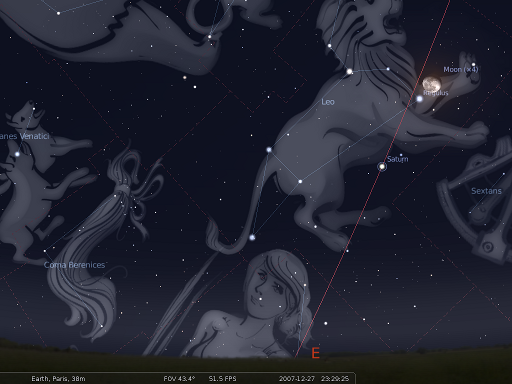
\includegraphics[width=0.9\textwidth]{002.png}
\caption{Night scene with constellation artwork and moon.}
\label{fig:002}
\end{figure}

Stellarium can do a whole lot more than just draw the stars. Figure~\ref{fig:002}
shows some of Stellarium's visual effects including constellation
line and boundary drawing, constellation art, planet hints, and
atmospheric halo around the bright Moon. The controls in the main tool bar
provide a mechanism for turning on and off the visual effects.

When the mouse is moved to the bottom left of the screen, a second
tool bar becomes visible. All the buttons in this side tool bar open
and close dialog boxes which contain controls for further
configuration of the program. The dialogs will be described in the
next chapter.


Table~\ref{tab:tour:buttons} describes the operations of buttons
on the main tool bar and the side tool bar, and gives their default
keyboard shortcuts.

%% TODO: Check default keys!
\newpage
%\begin{longtabu} to \textwidth {llcX}\toprule
\begin{longtable}{lccp{55mm}}\toprule
\emph{Feature}           & \emph{Button} & \emph{Hotkey} & \emph{Description}\\\midrule
Constellations           & \guibutton[0.75]{2.5}{bt_constellation.png}     & \key{C} & Draw constellations as ``stick figures'' \\
Constellation Names      & \guibutton[0.75]{2.5}{bt_constellation_name.png}& \key{V} & Draw name of the constellations \\
Constellation Art        & \guibutton[0.75]{2.5}{bt_constellation_art.png} & \key{R} & Superimpose artistic representations of the constellations \\
Constellation Boundaries & \guibutton[0.75]{2.5}{bt_constellation_boundaries.png}& \key{B} & Draw boundaries of the constellations\footnotemark[1]\\
Equatorial Grid          & \guibutton[0.75]{2.5}{bt_eq_grid.png}           & \key{E} & Draw grid lines for the equatorial coordinate system (RA/Dec) \\
Azimuth Grid             & \guibutton[0.75]{2.5}{bt_az_grid.png}           & \key{Z} & Draw grid lines for the horizontal coordinate system (Alt/Azi) \\
Galactic Grid            & \guibutton[0.75]{2.5}{bt_gal_grid.png}          &         & Draw grid lines for the galactic coordinate system (Long/Lat)\footnotemark[1]\\
Equatorial J2000 Grid    & \guibutton[0.75]{2.5}{bt_eq_j2000_grid.png}     &         & Draw grid lines for the equatorial coordinate system at standard epoch J2000.0 (RA/Dec) \footnotemark[1]\\
Ecliptic Grid            & \guibutton[0.75]{2.5}{bt_ecl_grid.png}          &         & Draw grid lines for the ecliptic coordinate system of date (Long/Lat)\footnotemark[1]\\
Toggle Ground            & \guibutton[0.75]{2.5}{bt_ground.png}            & \key{G} & Toggle drawing of the ground. Turn this off to see objects that are below the horizon. \\
Toggle Cardinal Points   & \guibutton[0.75]{2.5}{bt_cardinal.png}          & \key{Q} & Toggle marking of the North, South, East and West points on the horizon. \\
Toggle Compass Marks     & \guibutton[0.75]{2.5}{bt_compass_off.png}       & \key{\shift+Q} & Toggle degree marks along the horizon. \\
Toggle Atmosphere        & \guibutton[0.75]{2.5}{bt_atmosphere.png}        & \key{A} & Toggle atmospheric effects. Most notably makes the stars visible in the daytime.  \\
Deep-Sky Objects         & \guibutton[0.75]{2.5}{bt_nebulae.png}           & \key{D} & Toggle marking the positions of Deep-Sky Objects. \\
Planet Hints             & \guibutton[0.75]{2.5}{bt_planets.png}           & \key{P} & Toggle indicators to show the position of planets. \\
Nebula images            & \guibutton[0.75]{2.5}{bt_DSS.png}               & \key{I} & Toggle ``nebula images''.\footnotemark[1]\\
Digitized Sky Survey     & \guibutton[0.75]{2.5}{bt_ToastSurvey.png}       &  & Toggle ``Digitized Sky Survey'' (TOAST).\footnotemark[1]\\
Hierarchical Progressive Surveys & \guibutton[1.00]{2.5}{bt_Surveys.png}   & \key{\ctrl+Alt+D} & Toggle ``Hierarchical Progressive Surveys''.\footnotemark[1]\\
Coordinate System        & \guibutton[0.75]{2.5}{bt_coord_type.png}        & \key{\ctrl+M} & Toggle between horizontal (Alt/Azi) \& equatorial (RA/Dec) coordinate systems. \\
Center                   & \guibutton[0.75]{2.5}{bt_goto.png}              & \key{\Space} & Center the view on the selected object \\
Night Mode               & \guibutton[0.75]{2.5}{bt_night_mode.png}        & \key{\ctrl+N} & Toggle ``night mode'', which applies a red-only filter to the view to be easier on the dark-adapted eye. \\
Full Screen Mode         & \guibutton[0.75]{2.5}{bt_fullscreen.png}        & \key{F11} & Toggle full screen mode. \\
Bookmarks                & \guibutton[0.75]{2.5}{bt_bookmarks.png}         & \key{Alt+B} & Toggle bookmarks window.\footnotemark[1]\\
Flip view (horizontal)   & \guibutton[0.75]{2.5}{bt_fliph.png}      & \key{\ctrl+\shift+H} & Flip the image in the horizontal plane.\footnotemark[1] \\
Flip view (vertical)     & \guibutton[0.75]{2.5}{bt_flipv.png}      & \key{\ctrl+\shift+V} & Flip the image in the vertical plane.\footnotemark[1]\\
Quit Stellarium          & \guibutton[0.75]{2.5}{bt_quit.png}       & \key{\ctrl+Q} & Close Stellarium.\\
Help Window              & \guibutton[0.5]{2.5}{btd_help.png}       & \key{F1} & Show the help window, with key bindings and other useful information \\
Configuration Window     & \guibutton[0.5]{2.5}{btd_config.png}     & \key{F2} & Show the configuration window \\ 
Search Window            & \guibutton[0.5]{2.5}{btd_find.png}       & \key{F3} or \key{Ctrl+F} & Show the object search window \\
View Window              & \guibutton[0.5]{2.5}{btd_view.png}       & \key{F4} & Show the view window \\
Time Window              & \guibutton[0.5]{2.5}{btd_time.png}       & \key{F5} & Show the time window \\
Location Window          & \guibutton[0.5]{2.5}{btd_location.png}   & \key{F6} & Show the observer location window (map) \\
AstroCalc Window         & \guibutton[0.5]{2.5}{btd_astrocalc.png}  & \key{F10} & Show the astronomical calculations window \\
\bottomrule
\caption{Stellarium's standard menu buttons. Those marked \protect\footnotemark[1] must be enabled first, see section~\ref{sec:gui:configuration:tools}.}
\label{tab:tour:buttons}
\end{longtable}

\section{Taking Screenshots}
\label{sec:tour:screenshots}

You can save what is on the screen to a file by pressing
\key{\ctrl+S}. Screenshots are taken in PNG format, and have filenames
like \file{stellarium-000.png}, \file{stellarium-001.png} (the number
increments to prevent overwriting existing files). 

The screenshots are stored to a directory depending on your operating
system, see section~\ref{sec:Directories} Files and Directories.  See
also section~\ref{sec:gui:configuration:tools} for more screenshot options.

\section{Observing Lists (Bookmarks)}
\label{sec:tour:bookmarks}

You can store your favourite objects or views in observing lists. 
Press \key{Alt+B} or \guibutton[0.75]{2.5}{bt_bookmarks.png} to call
up the dialog.  A bookmarks file from previous versions will be
imported and converted to the new format. You can however create an
arbitrary number of lists. 

The list display shows all entries from the current list. A double
click on an entry selects the object.  To add an object to the list,
press \menu{Edit list}. This changes the view. Highlight (select)
your object in the sky and press \menu{Add object}. To remove an
object from a list, select its entry in the list and press
\menu{Remove object}. 

Sometimes storing the object alone is not enough. Interesting views like
planet conjunctions or eclipses require at least a time entry, if not
a particular location. Likewise, the displayed landscape may be nice
to restore. Additionally, the field of view may be relevant. To store
these data and later retrieve them, use the respective checkboxes.

You can also export the current list or all lists with the according
button, or import such an exported list on another system. 
To export the current list, keep the default \texttt{.sol} file type in the filename dialog.
To export all your lists, use the \texttt{.ol} file type in the filename dialog.
Lists are identified with an 
Universally Unique Identifier (UUID) which we call OLUD (Observing List Unique Identifier). 
On importing a list, existing lists with the same OLUD may be replaced after a warning. 
During editing, storing a list with an existing name is prevented. 
The list import may however import a list with an existing name as long as the OLUD is different. 
To transfer all your lists to another system, export them as \texttt{.ol} file, or
copy, rename and import (or just copy, to replace the existing) the full file \file{observingLists.json} 
from the \file{data/} subdirectory of your user directory (see section~\ref{sec:Directories}).


\section{Custom Markers}
\label{sec:tour:markers}

You can set temporary markers anywhere in the screen. These may be useful for various purposes but cannot be stored.

\begin{center}
\begin{tabular}{rl}\toprule
\emph{Actions}	                 & \emph{Description}\\\midrule
\key{Shift} \& left click        & Add custom marker \\
\key{Shift} \& right click       & Delete the one closest marker to mouse cursor\\
\key{Alt+\shift} \& right click  & Delete all custom markers 
\\\bottomrule
\end{tabular}
\end{center}

\section{Copy Information}
\label{sec:tour:copyInfo}

If you have selected an object and want to use the displayed
information elsewhere, you may want to copy it to the system clipboard
with \key{\ctrl+\shift+C}. In case you want to use its numbers
elsewhere, please see Appendix~\ref{ch:Accuracy} for known accuracy
limitations.


%%% Local Variables: 
%%% mode: latex
%%% TeX-master: "guide"
%%% End: 
